Let the boundary of the EB satisfy:

\begin{equation}
\label{eqn:billiard-f}
f(x,y)=\left(\frac{x}{a}\right)^2+\left(\frac{y}{b}\right)^2=1.
\end{equation}

Where $a>b>0$ denote the EB semi-axes throughout the paper. Below we use {\em aspect ratio} as the ratio of an ellipse's semi-axes. When referring to Triangle Centers we adopt Kimberling $X_i$ notation \cite{etc}, e.g., $X_1$ for the Incenter, $X_2$ for the Barycenter, etc., see Table~\ref{tab:kimberling} in Appendix~\ref{app:symbols}.

The following five-parameter equation is assumed for all circumconics not passing through $(0,0)$.

\begin{equation}
1 + c_1 x + c_2 y + c_3 x y + c_4 x^2 + c_5 y^2=0
\label{eqn:e0}
\end{equation}

\begin{proposition}
Any triangle $T=(P_1,P_2,P_3)$ is associated with a unique 
ellipse $E_9$ for which $T$ is a billiard 3-periodic. The center of $E_9$ is T's Mittenpunkt.
\end{proposition}

\begin{proof}
If $T$ is a 3-periodic of $E_9$, by Poncelet's Porism, $T$ is but an element of a 1d family of 3-periodics, all sharing the same confocal Caustic\footnote{This turns out to be the Mandart Inellipse $I_9$ of the family \cite{mw}.}. This family will share a common Mittenpunkt $X_9$ located at the center of $E_9$  \cite{reznik2020-intelligencer}. Appendix~\ref{app:circum-linear} shows how to obtain the parameters for \eqref{eqn:e0} such that it passes through $P_1,P_2,P_3$ and is centered on $X_9$: this yields a $5{\times}5$ linear system. Solving it its is obtained a quadratic equation with positive discriminant, hence the conic is an ellipse.
\end{proof}

$E_9$ is called the Circumbilliard (CB) of $T$. Figure~\ref{fig:circumbilliard} shows examples of CBs for two sample triangles.

\begin{figure}[H]
    \centering
    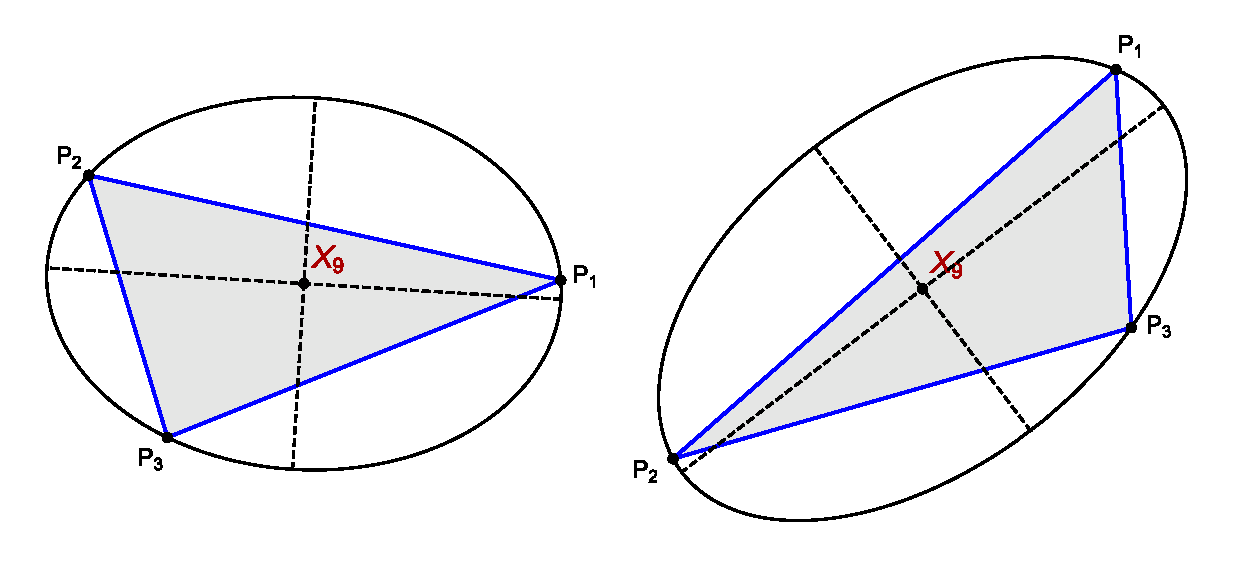
\includegraphics[width=.8\textwidth]{pics_eps_new/0010_circumplot}
    \caption{Two random triangles are shown as well as their Circumbilliards (CBs). Notice their axes in general are not horizontal/vertical. An algorithm for computing the CB is given in Appendix~\ref{app:circum-linear}. \textbf{Video:} \cite[PL\#02]{reznik2020-playlist-circum}}
    \label{fig:circumbilliard}
\end{figure}


